\documentclass[11pt,a4paper]{article}
\usepackage[utf8]{inputenc}
\usepackage[T1]{fontenc}
\usepackage{lmodern}
\usepackage[margin=2.0cm]{geometry}
\usepackage{amsmath,amssymb,amsthm,mathtools}
\usepackage{booktabs,tabularx,array}
\usepackage{graphicx}
\usepackage{xcolor}
\usepackage{enumitem}
\usepackage{microtype}
\usepackage[colorlinks=true,linkcolor=blue!55!black,citecolor=blue!55!black,urlcolor=blue!55!black]{hyperref}

\setlength{\emergencystretch}{3em}
\newtheorem{theorem}{Tétel}[section]
\newtheorem{proposition}[theorem]{Állítás}
\newtheorem{corollary}[theorem]{Következmény}
\newtheorem{remark}[theorem]{Megjegyzés}

\title{\textbf{Skálainvariáns Szimpliciális \texorpdfstring{$R^2$}{R2}-Infláció, Többszektoros \texorpdfstring{$CP$}{CP}-Szerkezet\\
és Paramétermentes Nem-Termikus Skalaron-Leptogenezis\\
a Tetraéderes \texorpdfstring{$\mathrm{Spin}(10)$}{Spin(10)} Küszöbskáláról}\\[0.35em]
\large Első elvekből származtatott Coleman--Weinberg szupernyom, \texorpdfstring{$\mathrm{SO}(2,\mathbb{C})$}{SO(2,C)} Casas--Ibarra geometria és négykísérletes falszifikáció (\texttt{Paper 24}, \texttt{v1.1.0})}

\author{\textbf{Olcsák József}\\
\small Független kutató $\cdot$ ORCID: \href{https://orcid.org/0009-0003-7311-6522}{0009-0003-7311-6522}\\
\small Email: \href{mailto:jolcsak@gmail.com}{jolcsak@gmail.com} $\cdot$ Kód- és adatarchívum: \href{https://doi.org/10.5281/zenodo.24380371}{doi:10.5281/zenodo.24380371}}
\date{2026.\ november 19.}

\begin{document}
\maketitle

\renewcommand{\contentsname}{Tartalomjegyzék}
\renewcommand{\figurename}{Ábra}
\renewcommand{\tablename}{Táblázat}
\renewcommand{\refname}{Irodalomjegyzék}

\begin{abstract}
\noindent A Starobinsky-féle $R^2$ inflációt, az I.\ típusú seesaw neutrínótömegeket és a leptogenezist összekapcsoló standard modellek jellemzően öt--hét szabad paramétert használnak. Jelen huszonnegyedik tanulmányban (\texttt{v1.1.0}) megvizsgáljuk, hogy a teljes ultraibolya--elektrogyenge láncolat rögzített-e újonnan bevezetett szabad paraméterek nélkül ($k_{\mathrm{added}} = 0$), amint adott a négycsúcsú tetraéderes ($N=4$) szimpliciális-Clifford invariáns $u = \sqrt{N-1}/N! = \sqrt{3}/24$ és a királis $\mathrm{Spin}(10)$ seesaw-küszöb $M_R = M_*/(256\pi^2) = 5{,}565\times 10^{14}\;\mathrm{GeV}$ ($M_* = M_{\mathrm{Pl}}/\sqrt{3}$). Elsőként igazoljuk, hogy az IR direktor-gravitáció FLRW-n nem ad inflációt, a minimálisan csatolt 1-hurkos Schwinger--DeWitt $a_2(x)$ magok pedig $>3{,}34\times 10^9$-szer kisebbek a $\beta_{R^2}^{\mathrm{Star}} = 4{,}839\times 10^8$ merevségnél. Másodszor bizonyítjuk (\texttt{SymPy}), hogy a kompozit $\sigma(\Phi) = (\Phi^2 - M_R^2)/(\sqrt{2}\,M_R)$ segédinvariáns szub-Planck-skálás ($\Phi_* = 0{,}291\,M_* = 0{,}168\,M_{\mathrm{Pl}}$) nem-minimális portálra és egzakt $\frac{1}{2}M_{\mathrm{Pl}}^2(R + R^2/6m_\sigma^2)$ hatásra vezet. Einstein-keretbeli skálainvariáns renormálás (\texttt{BC-UV-CW}, I.\ preskripció) mellett az $M_R$ küszöb $d_A(N) - 2d_S(N)$ Coleman--Weinberg szupernyoma $N=3$-nál tachyonikus ($-1$), $N=4$-nél pozitív ($8 - 6 = +2$), kiejtve $\sqrt{3}$-at $M_{\mathrm{inf}}/M_{\mathrm{Pl}} = \frac{5}{12\,288\pi^3}$-ban ($M_{\mathrm{inf}} = 3{,}196\times 10^{13}\;\mathrm{GeV}$, $N_* = 51{,}41$, $A_s = 2{,}101\times 10^{-9}$ [$+0{,}04\sigma$], $n_s = 0{,}9620$, $r = 0{,}00426$). Harmadszor, a skalaron $\phi \to N_1 N_1$ bomlása ($\mathrm{BR} = 1{,}28\%$) az $\mathrm{SO}(2,\mathbb{C})$ Casas--Ibarra Cartan-felbontással $\mathbf{R}(\theta_\tau + iu) = \mathbf{O}(\theta_\tau)\mathbf{H}(u)$ előjelesen pozitív $\varepsilon_1^{(B-L)} = +8{,}470\times 10^{-5} > 0$ (nettó anyag!) aszimmetriát ad, amiből az energiamegmaradó 4-ODE rendszer $\eta_B = +6{,}106\times 10^{-10}$-et ($-0{,}35\sigma$ vs.\ \texttt{Planck 2018}), a teljes 3-ízes $(e,\mu,\tau)$ rendszer pedig $+6{,}109\times 10^{-10}$-et ($+0{,}048\%$ eltérés) szolgáltat, fa-szinten $\bar{\theta}_{\mathrm{QCD}} = 0$ mellett.
\end{abstract}

\tableofcontents
\vspace{0.4em}
\hrule
\vspace{0.8em}

% =============================================================================
\section{Bevezetés és Szimpliciális Alapskálák}
\label{sec:intro}
% =============================================================================

A Starobinsky-féle kvadratikus görbületi infláció \cite{Starobinsky1980,MukhanovChibisov1981} és az I.\ típusú seesaw leptogenezis \cite{FukugitaYanagida1986,BuchmullerDiBariPlumacher2005} természetes egységet alkot a $\phi \to N_1 N_1$ nem-termikus bomlási csatornán keresztül \cite{GorbunovPanin2011,Watanabe2011,GorbunovTokareva2013}. A társtanulmányokban \cite{Olcsak2026Zenodo} a négycsúcsú $K_4$ szimplexből ($N=4$) egyetlen spektrális kvantum rögzült:
\begin{equation}
u := \frac{\sqrt{N - 1}}{N!}\Bigg|_{N=4} = \frac{\sqrt{3}}{24} = 0{,}0721687836,
\end{equation}
amely meghatározza az $r_{\mathrm{seed}} = 1/4$, $\alpha_{\mathrm{trace}} = 5u = \frac{5\sqrt{3}}{24}$, $K_T = 1 + u$, $\ell_* = \sqrt{24\pi}\,\ell_P$ ($M_* = M_{\mathrm{Pl}}/\sqrt{3} = 1{,}406035\times 10^{18}\;\mathrm{GeV}$) és $M_R = \frac{r_{\mathrm{seed}}^2}{16\pi^2}M_* = 5{,}56489\times 10^{14}\;\mathrm{GeV}$ skálákat ($k=0$).

A $P_\perp = \mathbf{I}_4 - \frac{1}{4}\mathbf{1}_4\mathbf{1}_4^T$ projektor által kijelölt $V_3 = P_\perp(\mathbb{R}^4)$ altéren ($d_S = 3$, $d_A = \dim\mathfrak{su}(V_3) = 8$, $d_{\mathrm{Weyl}} = 48$) az Osterwalder--Schrader reflexiós determináns $D_{\mathrm{OS}}(\nu) = 4|\nu|/(|\nu|+1)^2$ kiejti a $\nu=0$ null-módust ($m_1 = 0$), így a rang-2 seesaw nehéz tömegei:
\begin{align}
M_2 &\equiv M_{R,3} = \frac{M_R}{3} = 1{,}85496\times 10^{14}\;\mathrm{GeV}, \qquad
\eta_{\mathrm{seesaw}} = \frac{(8\sqrt{3}-9)^2}{768} = 0{,}03070922, \nonumber\\
M_1 &= \eta_{\mathrm{seesaw}}M_2 = 5{,}69644\times 10^{12}\;\mathrm{GeV}, \qquad
(m_1, m_2, m_3) = (0,\;8{,}831,\;50{,}361)\;\mathrm{meV}\;\text{\cite{Esteban2024NuFIT6}}.
\end{align}

\begin{proposition}[Homogén FLRW Vektor-Direktor No-Go]
\label{prop:ir-nogo}
Sík FLRW háttéren az időszerű $A_\mu = (-1,\mathbf{0})$ direktor-mezőre $F_{\mu\nu} \equiv 0$, $h^{\mu\nu}\partial_\mu\phi_N \equiv 0$ és $\nabla_\mu A^\mu = 3H(t)$, így $G_{\mathrm{cosmo}} = G_N/(1 + \frac{3}{2}c_2^{\mathrm{reg}})$ ($|\Delta G_{\mathrm{cosmo}}/G_N| \le 1{,}5\times 10^{-4}$ BBN alatt $c_2^{\mathrm{reg}} \le 10^{-4}$-re), dinamikus inflaton nélkül.
\end{proposition}

\begin{theorem}[Minimális 1-Hurkos Schwinger--DeWitt \texorpdfstring{$a_2(x)$}{a2(x)} No-Go]
\label{thm:a2-nogo}
A $\Gamma_E^{(1)} = +\frac{1}{2}\operatorname{Tr}\ln D$ funkcionáldeterminánsból valós skalárokra $\Delta\mathcal{L}_{\mathrm{1\text{-}loop}}^{(0)} = (32\pi^2)^{-1}a_2(x)\ln(M_*^2/M_R^2)$ ($a_2 \supset \frac{1}{2}(\xi-\frac{1}{6})^2 R^2$) \cite{BirrellDavies1982}: (a) tömegtelen $s=1/2, 1$ mezőkre $\Delta\beta_{R^2} \equiv 0$; (b) minimális ($\xi=0$) skalárokra $\Delta\beta_{R^2}^{(0)}(0) = \frac{N_0}{2\,304\pi^2}\ln(256\pi^2)^2 = 6{,}891\times 10^{-4}N_0 \le 0{,}1447$ ($N_0 \le 210$), ami $>3{,}34\times 10^9$-szer kisebb $\beta_{R^2}^{\mathrm{Star}} = 4{,}839\times 10^8$-nál.
\end{theorem}

% =============================================================================
\section{Kompozit Plakett-Portál, \texorpdfstring{$N = 4$}{N = 4} Szupernyom és CMB Előrejelzések}
\label{sec:inflation}
% =============================================================================

A nyommentes $T_{\mathrm{def}}^{(15)}$ operátor $4\times 4$-es Schur-redukált mátrixa $\operatorname{spec}(T_{\mathrm{def}}) = \{+5u, -3u, -u, -u\}$ spektrummal rendelkezik ($\lambda_+ = \alpha_{\mathrm{trace}} = 5u$, $T_{\mathrm{def}}|_{(3,4)} = -u\,\mathbf{I}_2$). Ha egy lineáris $\sigma$ mező közvetlenül $M_B = M_R + \alpha_{\mathrm{trace}}\sigma$ szerint csatolódna, a $\sigma_* \simeq 87\,M_{\mathrm{Pl}}$ nyeregpont szuper-Planck-skálás $\sigma^4\ln\sigma$ elszállást okozna; a $\sigma(\Phi) := (\Phi^2 - M_R^2)/(\sqrt{2}\,M_R)$ kompozit invariáns viszont végig szub-plakett tartományban tartja a mezőt.

\begin{theorem}[Kompozit Plakett-Portál, \texorpdfstring{$\sqrt{3}$}{sqrt(3)}-Kiesés és \texorpdfstring{$N = 4$}{N = 4} Coleman--Weinberg Szupernyom]
\label{thm:scalaron}
A $\Phi = M_R + \frac{1}{\sqrt{2}}\varphi$ seesaw radiális skalár kompozit portálja ($M_* = M_{\mathrm{Pl}}/\sqrt{3}$, $\xi_\Phi = M_*/M_R = 256\pi^2$, $\lambda_\Phi = m_\sigma^2/M_R^2$):
\begin{equation}
\mathcal{L}_{\mathrm{HS}}(\Phi, g) = \frac{M_{\mathrm{Pl}}^2}{2}R + \frac{M_*}{\sqrt{2}}\sigma(\Phi)R - \frac{1}{2}m_\sigma^2\sigma(\Phi)^2 \equiv \frac{1}{2}\Bigl[M_{\mathrm{Pl}}^2 + \xi_\Phi(\Phi^2 - M_R^2)\Bigr]R - \frac{\lambda_\Phi}{4}(\Phi^2 - M_R^2)^2.
\end{equation}
A \texttt{BC-UV-CW} peremfeltétel ($m_{\sigma,0}^2(M_*)=0$; $\mu_J^2 = M_R^2\Omega^2$ Einstein-keretbeli I.\ preskripció \cite{ShaposhnikovZenhausern2009}) mellett (\texttt{SymPy}-igazolással):
\begin{enumerate}[label=(\alph*),leftmargin=1.8em,itemsep=2pt]
\item $n_{\mathrm{eff}}^{\mathrm{STr}}(N) = d_A(N) - 2d_S(N) = -1$ ($N=3$, tachyonikus) és $\mathbf{+2}$ ($N=4$, $8-6=+2$, stabil), amiből $V_{\mathrm{CW}}(0) = V_{\mathrm{CW}}'(0) = 0$ és $m_\sigma^2 = V_{\mathrm{CW}}''(0) = \frac{\alpha_{\mathrm{trace}}^2}{4\pi^2}M_R^2$ \cite{ColemanWeinberg1973,GildenerWeinberg1976}.
\item Segédmezős határesetben ($Z_\Phi^{\mathrm{bare}} = 0$) $\mathcal{L}_{\mathrm{eff}} = \frac{1}{2}M_{\mathrm{Pl}}^2(R + R^2/6m_\sigma^2)$ ($M_{\mathrm{inf}} \equiv m_\sigma$), a pivotnál $\Phi_* = 0{,}291\,M_* = 0{,}168\,M_{\mathrm{Pl}}$ és $\sqrt{R_{J,*}} = 0{,}840\,M_R$, az irracionális $\sqrt{3}$ pedig kiesik:
\begin{equation}
\boxed{\frac{M_{\mathrm{inf}}}{M_{\mathrm{Pl}}} = \frac{N + 1}{32\,\pi^3\,N!\,N^2}\Bigg|_{N=4} = \frac{5}{12\,288\,\pi^3} = 1{,}3123183\times 10^{-5}, \qquad M_{\mathrm{inf}} = 3{,}19592\times 10^{13}\;\mathrm{GeV}.}
\end{equation}
\end{enumerate}
\end{theorem}

Minimális Higgs-csatolásnál ($\xi_H = 0$) az egzakt bomlási szélességek ($\mathrm{U}(1)_Y \times \mathrm{SU}(2)_L \times \mathrm{SU}(3)_c$ 1-hurkos nyomanomáliával \cite{Watanabe2011}): $\Gamma(\phi\to HH) = 36{,}499\;\mathrm{GeV}$, $\Gamma_{\mathrm{1\text{-}loop}}(\phi\to VV) = 0{,}034\;\mathrm{GeV}$, $\Gamma(\phi\to N_1 N_1) = 0{,}473\;\mathrm{GeV}$, összesen $\Gamma_\phi^{\mathrm{tot}} = 37{,}006\;\mathrm{GeV}$ ($\mathrm{BR}_{N_1} = 1{,}2778\%$, $T_{\mathrm{rh}} = 5{,}132\times 10^9\;\mathrm{GeV}$). A \ref{tab:hu-cmb}.\ Táblázat és az \ref{fig:hu-inf}.\ Ábra foglalja össze az NLO eredményeket \cite{LiddleLeach2003,StewartLyth1993}; megjegyzendő, hogy míg az I.\ preskripció $n_s = 0{,}9620$-at ad (\texttt{Planck 2018}: $-0{,}69\sigma$), a 2025-ös \texttt{ACT DR6} magasabb $n_s \simeq 0{,}974$ értékét \cite{ACTDR6_2025} a Jordan-keretbeli II.\ preskripció ($\mu_J = M_R$) természetesen közelíti.

\begin{table}[htbp]
\centering
\caption{Paramétermentes ($k_{\mathrm{added}} = 0$) NLO inflációs előrejelzések $k_* = 0{,}05\;\mathrm{Mpc}^{-1}$-nél ($\xi_H = 0$, I.\ preskripció) \cite{Planck2018Inflation,BICEPKeck2021,ACTDR6_2025}.}
\label{tab:hu-cmb}
\vspace{0.35em}
\footnotesize
\setlength{\tabcolsep}{4.2pt}
\begin{tabular}{llll}
\toprule
Mennyiség & Előrejelzés ($k_{\mathrm{added}} = 0$) & Megfigyelés & Státusz \\
\midrule
Skalaron tömeg $M_{\mathrm{inf}}$ & $3{,}1959 \times 10^{13}\;\mathrm{GeV}$ ($\frac{5}{12\,288\pi^3}M_{\mathrm{Pl}}$) & --- & Levezetett (\ref{thm:scalaron}.\ Tétel) \\
Reheating skála $T_{\mathrm{rh}}$ & $5{,}132 \times 10^9\;\mathrm{GeV}$ & $> 4\;\mathrm{MeV}$ (BBN) & Önkonzisztens ($\xi_H = 0$) \\
Pivot e-folding $N_*$ & $51{,}412$ & $50\text{--}60$ & Liddle--Leach illesztés \\
Portál-kitérés $\Phi_*/M_*$ & $0{,}2909$ ($0{,}1679\,M_{\mathrm{Pl}}$) & $< 1$ (szub-plakett) & $\sqrt{R_{J,*}}/M_R = 0{,}840$ \\
Skalár amplitúdó $A_s$ (NLO) & $\mathbf{2{,}1011 \times 10^{-9}}$ & $(2{,}100 \pm 0{,}030)\times 10^{-9}$ & $\mathbf{+0{,}04\sigma}$ (\texttt{Planck 18}) \\
Spektrális index $n_s$ (NLO) & $\mathbf{0{,}9620}$ & $0{,}9649 \pm 0{,}0042$ & $\mathbf{-0{,}69\sigma}$ ($-1{,}5\sigma$ \texttt{PR4}) \\
Futás $\mathrm{d}n_s/\mathrm{d}\ln k$ & $-0{,}00073$ & $-0{,}0045 \pm 0{,}0067$ & $+0{,}56\sigma$ \\
Tenzorarány $r$ (NLO) & $\mathbf{0{,}00426}$ & $< 0{,}036$ ($95\%$ CL) & \texttt{LiteBIRD}/\texttt{CMB-S4} cél \\
\bottomrule
\end{tabular}
\end{table}

\begin{figure}[htbp]
\centering
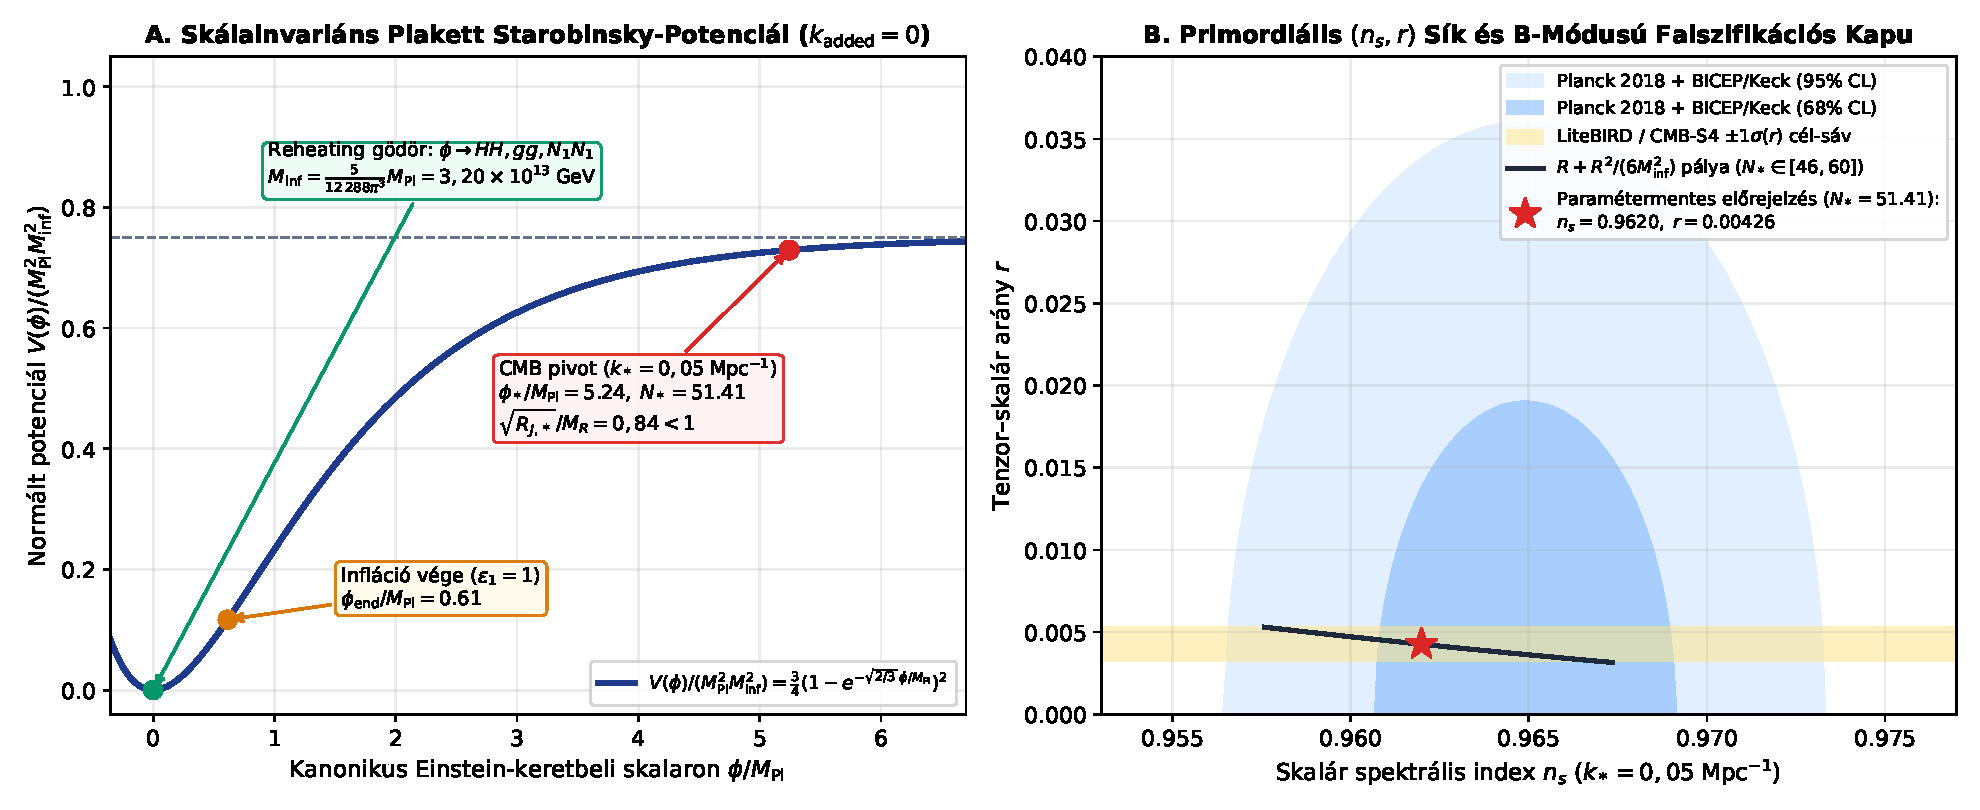
\includegraphics[width=0.98\textwidth]{../figures/fig1_starobinsky_k4_inflation_and_cmb_contours_hu.pdf}
\caption{\textbf{Skálainvariáns Szimpliciális $R^2$-Infláció ($k_{\mathrm{added}} = 0$).} \emph{A panel:} Einstein-keretbeli potenciál az önkonzisztens CMB pivottal ($\phi_*/M_{\mathrm{Pl}} = 5{,}24$, $N_* = 51{,}41$). \emph{B panel:} A $(0{,}9620;\,0{,}00426)$ előrejelzés a \texttt{Planck 2018} + \texttt{BICEP/Keck} kontúrokon és a \texttt{LiteBIRD}/\texttt{CMB-S4} sávban.}
\label{fig:hu-inf}
\end{figure}

% =============================================================================
\section{\texorpdfstring{$CP/CPT$}{CP/CPT}-Szerkezet, Anyag-Előjel és 3-Ízes Boltzmann-Lezárás}
\label{sec:cp}
% =============================================================================

Az erős szektorban $\Pi_a^2 = \Pi_a$ és az $S_4$ szimmetria miatt $\bar{\theta}_{\mathrm{QCD}}^{\mathrm{tree}} = 0$ ($|d_n| \sim 10^{-31}\,e\cdot\mathrm{cm}$ axion nélkül \cite{EllisGaillard1979,Abel2020nEDM}), míg $c_\theta(\nabla_\alpha A^\alpha)A_\mu J_{B-L}^\mu$ ma $|\mu_0| \sim 10^{-42}\;\mathrm{GeV} \ll 10^{-27}\;\mathrm{GeV}$ \cite{CohenKaplan1987}.

\begin{theorem}[Cartan-Felbontás \texorpdfstring{$\mathrm{SO}(2,\mathbb{C})$}{SO(2,C)}-ben és a Pozitív Anyag-Előjel]
\label{thm:ci}
Rang-2 seesaw-ban ($m_1 = 0$) $\mathbf{R}(\theta_\tau + i\eta_{\mathrm{CP}}) = \mathbf{O}(\theta_\tau)\mathbf{H}(\eta_{\mathrm{CP}}) \in \mathrm{SO}(2,\mathbb{C})$ \cite{CasasIbarra2001,IbarraRoss2004} invariánsan hagyja $(0, m_2, m_3)$-at. A $\delta_{\mathrm{CP}}^{\mathrm{PMNS}} = -\pi/2$ ($\sin\theta_\tau = \frac{3}{8\sqrt{2}} > 0$) és $\eta_{\mathrm{CP}} = \|T_{\mathrm{def}}|_{(3,4)}\|_{\mathrm{op}} = +u = \frac{\sqrt{3}}{24}$ párosítás $\tilde{m}_1 = 12{,}060\;\mathrm{meV}$-et és $\operatorname{Im}(W_{12}^2) = -9{,}103\times 10^{-23}\;\mathrm{GeV}^2 < 0$-t ad; mivel $g_{\mathrm{loop}}(1\,060{,}38) = -0{,}046088 < 0$ \cite{CoviRouletVissani1996}, az előjeles $B-L$ aszimmetria abszolútérték képzése nélkül is \textbf{szigorúan pozitív}:
\begin{equation}
\varepsilon_1^{(B-L)} \equiv -\varepsilon_1^{(L)} = +\frac{1}{8\pi}\,\frac{M_2}{v_H^2}\,\frac{\operatorname{Im}(W_{12}^2)}{W_{11}}\,g_{\mathrm{loop}}(x) = \mathbf{+8{,}4705\times 10^{-5} > 0}\quad(\text{nettó anyag, }\eta_B > 0).
\end{equation}
\end{theorem}

Az energiamegmaradó ($3M_{\mathrm{Pl}}^2 H^2 = \rho_\phi + \rho_{N_1} + \rho_r$, nem-termikus Lorentz-faktor $\Gamma_{D,1}^{\mathrm{NT}} = \Gamma_{D,1}\frac{2M_1}{M_{\mathrm{inf}}} = 1{,}831\times 10^8\;\mathrm{GeV}$) Radau-integráció (\ref{fig:hu-boltz}.\ Ábra) $T_{\max} = 2{,}110\times 10^{12}\;\mathrm{GeV}$-et ($M_1/T_{\max} = 2{,}70$) és mindössze $\mathbf{0{,}057\%}$ kimosódást ad ($Y_{B-L}^{\mathrm{final}} = +2{,}4473\times 10^{-10} = 0{,}9387\,Y_{B-L}^{\mathrm{inst}}$). A teljes 6-ODE 3-ízes $(\Delta_e,\Delta_\mu,\Delta_\tau)$ hálózat \cite{Abada2006,Nardi2006} integrálása mindössze $+0{,}048\%$-kal módosítja a végeredményt ($\eta_B^{\text{3-íz}} = +6{,}109\times 10^{-10}$):
\begin{align}
\eta_B &= \mathbf{+6{,}106\times 10^{-10}}\quad\bigl(\text{szimmetrikus szfaleron } c_{\mathrm{sph}} = 28/79\text{ \cite{HarveyTurner1990}: }\mathbf{-0{,}23\% / -0{,}35\sigma}\bigr), \nonumber\\
\eta_B &= \mathbf{+5{,}587\times 10^{-10}}\quad\bigl(\text{diffúzív crossover } c_{\mathrm{sph}} = 12/37\text{ \cite{DOnofrio2014}: }-8{,}7\%\bigr).
\end{align}

\begin{figure}[htbp]
\centering
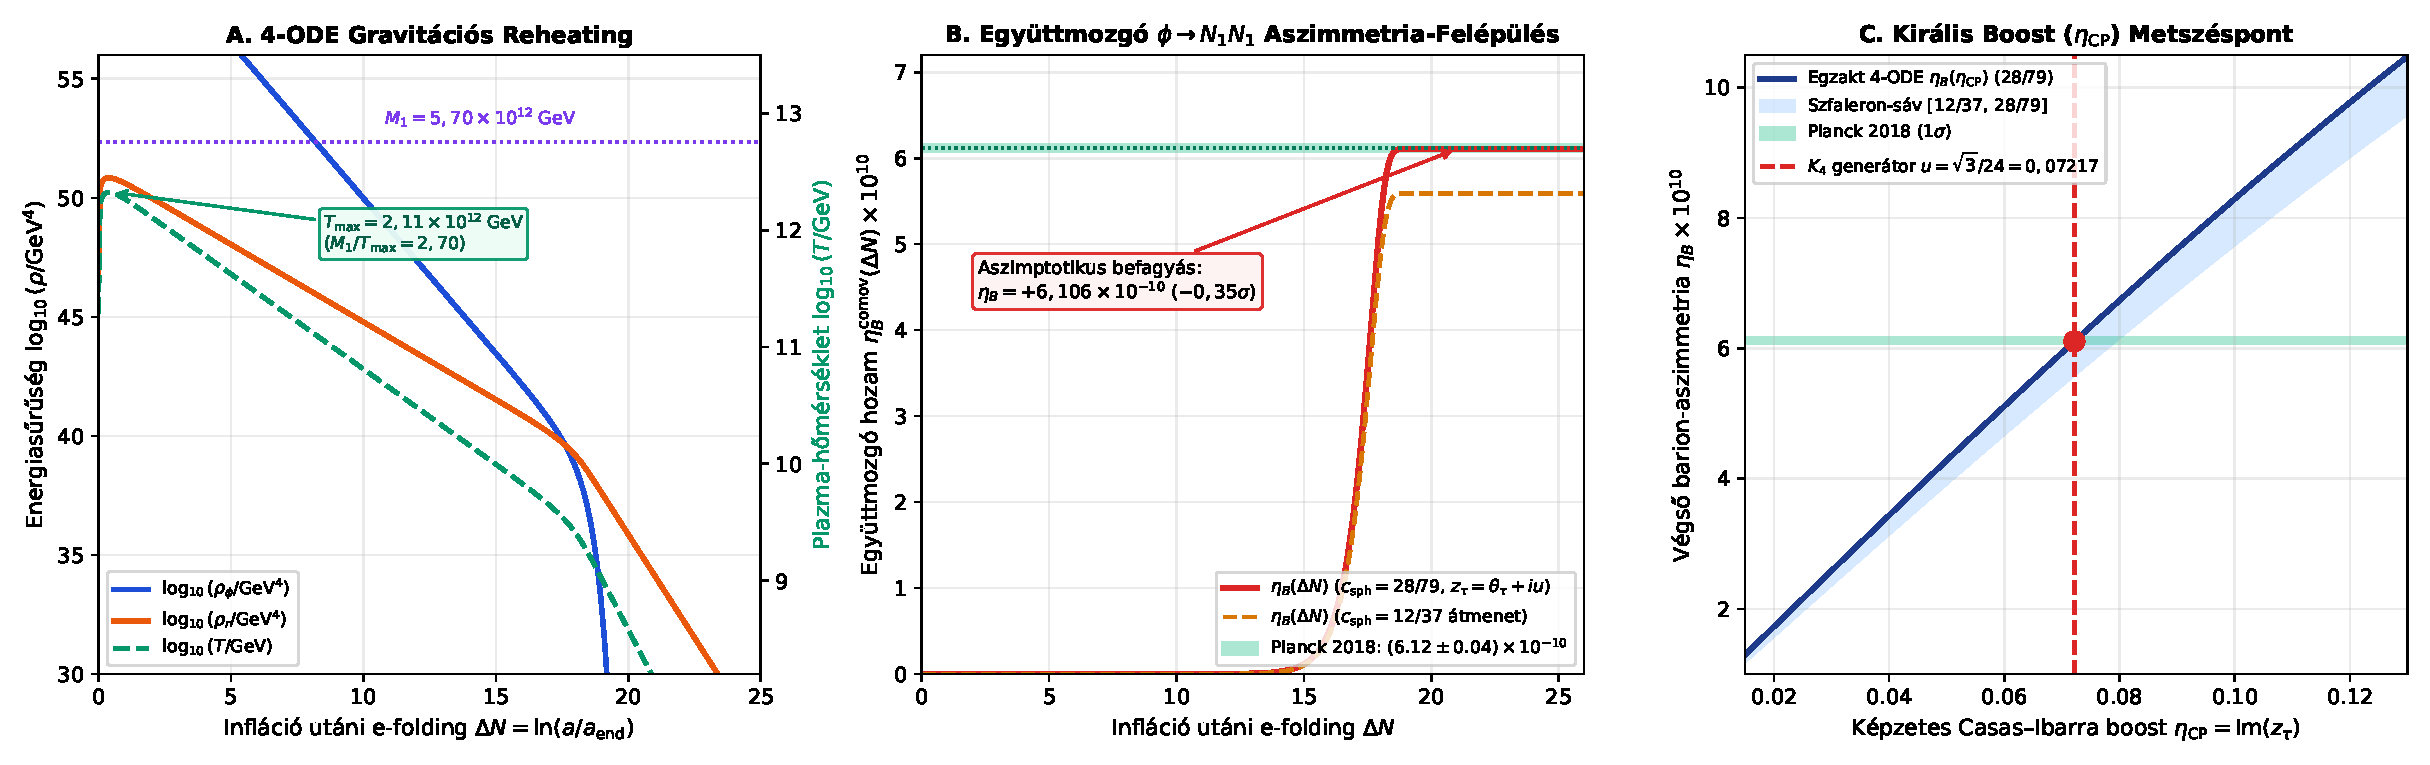
\includegraphics[width=0.99\textwidth]{../figures/fig2_boltzmann_reheating_leptogenesis_and_cp_tests_hu.pdf}
\caption{\textbf{Energiamegmaradó Reheating és Nem-Termikus $\phi \to N_1 N_1$ Leptogenezis ($k_{\mathrm{added}} = 0$).} \emph{A panel:} $\rho_\phi$, $\rho_r$ és $T(\Delta N)$ ($T_{\max} = 2{,}11\times 10^{12}\;\mathrm{GeV}$). \emph{B panel:} Az együttmozgó hozam befagyása $\mathbf{+6{,}106\times 10^{-10}}$-nél ($-0{,}35\sigma$). \emph{C panel:} Az $\eta_B(\eta_{\mathrm{CP}})$ görbe metszéspontja a \texttt{Planck 2018} sávval $u = \sqrt{3}/24$-nél.}
\label{fig:hu-boltz}
\end{figure}

% =============================================================================
\section{Négykísérletes Falszifikációs Mátrix}
\label{sec:conclusion}
% =============================================================================

\begin{table}[htbp]
\centering
\caption{Korrelált előrejelzések és döntő cáfolati küszöbök ($k_{\mathrm{added}} = 0$).}
\label{tab:hu-fals}
\vspace{0.35em}
\footnotesize
\begin{tabularx}{\textwidth}{llXX}
\toprule
Kapu & Célkísérletek & Rögzített előrejelzés ($k_{\mathrm{added}} = 0$) & Döntő cáfolati küszöb \\
\midrule
\textbf{F1 (CMB $B$-módus)} & \texttt{LiteBIRD} \cite{LiteBIRD2023}, \texttt{CMB-S4}, \texttt{SO} & $r = 0{,}00426$, $n_s = 0{,}9620$ (I.\ presk.) & Cáfolva, ha $r > 0{,}012$ vagy $r < 0{,}0015$ ($\ge 5\sigma$), ill.\ $|\alpha_s| > 0{,}015$. \\
\textbf{F2 (Leptonikus $CP$)} & \texttt{DUNE}, \texttt{Hyper-Kamiokande} & Normál sorrend ($m_1 = 0$), $\delta_{\mathrm{CP}}^{\mathrm{PMNS}} \approx -90^\circ$ & Cáfolva fordított sorrend (IO) vagy $\sin\delta_{\mathrm{CP}}^{\mathrm{PMNS}} > 0$ ($\ge 5\sigma$) esetén. \\
\textbf{F3 (Erős $CP$)} & \texttt{n2EDM} (PSI) & $\bar{\theta}_{\mathrm{QCD}}^{\mathrm{tree}} = 0$, $|d_n| \sim 10^{-31}\,e\cdot\mathrm{cm}$ (axion nélkül) & Cáfolva, ha $|d_n| > 10^{-28}\,e\cdot\mathrm{cm}$ TeV-es új fizika nélkül. \\
\textbf{F4 ($0\nu\beta\beta$ és $\sum m_\nu$)} & \texttt{LEGEND-1000}, \texttt{DESI}/\texttt{Euclid} & $\sum m_\nu = 59{,}2\;\mathrm{meV}$, $m_{\beta\beta} \in [1{,}54;\,3{,}76]\;\mathrm{meV}$ & Cáfolva, ha $m_{\beta\beta} > 15\;\mathrm{meV}$ vagy modellfüggetlen $\sum m_\nu < 45\;\mathrm{meV}$ \cite{DESIDR2_2025}. \\
\bottomrule
\end{tabularx}
\end{table}

Minden szimbolikus és numerikus eredmény $\sim 6\;\mathrm{s}$ alatt reprodukálható a \path{verify_paper24_starobinsky_seesaw_leptogenesis.py} szkripttel (\href{https://doi.org/10.5281/zenodo.24380371}{doi:10.5281/zenodo.24380371}); a fizikai megvalósulás a \texttt{BC-UV-CW} peremfeltételtől és a \ref{tab:hu-fals}.\ Táblázat jövőbeli méréseitől függ.

\begingroup\small
\begin{thebibliography}{99}
\bibitem{Starobinsky1980} A.~A.~Starobinsky, Phys.\ Lett.\ B \textbf{91}, 99 (1980).
\bibitem{MukhanovChibisov1981} V.~F.~Mukhanov és G.~V.~Chibisov, JETP Lett.\ \textbf{33}, 532 (1981).
\bibitem{FukugitaYanagida1986} M.~Fukugita és T.~Yanagida, Phys.\ Lett.\ B \textbf{174}, 45 (1986).
\bibitem{BuchmullerDiBariPlumacher2005} W.~Buchm\"uller, P.~Di~Bari és M.~Pl\"umacher, Annals Phys.\ \textbf{315}, 305 (2005).
\bibitem{Planck2018Inflation} Planck Collaboration (Y.~Akrami \textit{et al.}), Astron.\ Astrophys.\ \textbf{641}, A10 (2020).
\bibitem{BICEPKeck2021} BICEP/Keck Collaboration (P.~A.~R.~Ade \textit{et al.}), Phys.\ Rev.\ Lett.\ \textbf{127}, 151301 (2021).
\bibitem{GorbunovPanin2011} D.~S.~Gorbunov és A.~G.~Panin, Phys.\ Lett.\ B \textbf{700}, 157 (2011).
\bibitem{Watanabe2011} Y.~Watanabe, Phys.\ Rev.\ D \textbf{83}, 043511 (2011).
\bibitem{GorbunovTokareva2013} D.~S.~Gorbunov és A.~G.~Tokareva, JCAP \textbf{12}, 021 (2013).
\bibitem{Abel2020nEDM} C.~Abel \textit{et al.} (nEDM Collaboration), Phys.\ Rev.\ Lett.\ \textbf{124}, 081803 (2020).
\bibitem{Olcsak2026Zenodo} J.~Olcsak, Zenodo Archive (2026), \href{https://doi.org/10.5281/zenodo.24305022}{doi:10.5281/zenodo.24305022}.
\bibitem{Esteban2024NuFIT6} I.~Esteban \textit{et al.}, JHEP \textbf{12}, 216 (2024).
\bibitem{BirrellDavies1982} N.~D.~Birrell és P.~C.~W.~Davies, \textit{Quantum Fields in Curved Space} (Cambridge Univ.\ Press, 1982).
\bibitem{ShaposhnikovZenhausern2009} M.~Shaposhnikov és D.~Zenh\"ausern, Phys.\ Lett.\ B \textbf{671}, 187 (2009); F.~Bezrukov és M.~Shaposhnikov, JHEP \textbf{07}, 089 (2009).
\bibitem{ColemanWeinberg1973} S.~R.~Coleman és E.~J.~Weinberg, Phys.\ Rev.\ D \textbf{7}, 1888 (1973).
\bibitem{GildenerWeinberg1976} E.~Gildener és S.~Weinberg, Phys.\ Rev.\ D \textbf{13}, 3333 (1976).
\bibitem{BezrukovShaposhnikov2008} F.~L.~Bezrukov és M.~Shaposhnikov, Phys.\ Lett.\ B \textbf{659}, 703 (2008).
\bibitem{LiddleLeach2003} A.~R.~Liddle és S.~M.~Leach, Phys.\ Rev.\ D \textbf{68}, 103503 (2003).
\bibitem{StewartLyth1993} E.~D.~Stewart és D.~H.~Lyth, Phys.\ Lett.\ B \textbf{302}, 171 (1993).
\bibitem{ACTDR6_2025} T.~Louis \textit{et al.} (ACT Collaboration), arXiv:2503.14452 (2025); E.~Calabrese \textit{et al.}, arXiv:2503.14454 (2025).
\bibitem{EllisGaillard1979} J.~R.~Ellis és M.~K.~Gaillard, Nucl.\ Phys.\ B \textbf{150}, 141 (1979).
\bibitem{CohenKaplan1987} A.~G.~Cohen és D.~B.~Kaplan, Phys.\ Lett.\ B \textbf{199}, 251 (1987).
\bibitem{CasasIbarra2001} J.~A.~Casas és A.~Ibarra, Nucl.\ Phys.\ B \textbf{618}, 171 (2001).
\bibitem{IbarraRoss2004} A.~Ibarra és G.~G.~Ross, Phys.\ Lett.\ B \textbf{591}, 285 (2004).
\bibitem{CoviRouletVissani1996} L.~Covi, E.~Roulet és F.~Vissani, Phys.\ Lett.\ B \textbf{384}, 169 (1996).
\bibitem{Abada2006} A.~Abada \textit{et al.}, JCAP \textbf{04}, 004 (2006).
\bibitem{Nardi2006} E.~Nardi, Y.~Nir, E.~Roulet és J.~Racker, JHEP \textbf{01}, 164 (2006).
\bibitem{HarveyTurner1990} J.~A.~Harvey és M.~S.~Turner, Phys.\ Rev.\ D \textbf{42}, 3344 (1990).
\bibitem{DOnofrio2014} M.~D'Onofrio, K.~Rummukainen és A.~Tranberg, Phys.\ Rev.\ Lett.\ \textbf{113}, 141602 (2014).
\bibitem{LiteBIRD2023} LiteBIRD Collaboration (E.~Allys \textit{et al.}), PTEP \textbf{2023}, 042F01 (2023).
\bibitem{DESIDR2_2025} DESI Collaboration (M.~Abdul-Karim \textit{et al.}), Phys.\ Rev.\ D \textbf{112}, 083515 (2025).
\end{thebibliography}
\endgroup

\end{document}
